\section{Baby-steps/Giant-steps algorithm (Shank's method)}
\begin{itemize}
    \item Let $p$ be a large prime number.
    \item Let also $\mathbb{Z}_{p}^{*} = <g> = \{1, \dots, p-1\}$.
    \item Let $x \in \mathbb{Z}_{p}^{*}$.
    \item The goal is to find $y$ such that $x = g^{y} \bmod p$.
\end{itemize}
The algorithm proceeds as follows:
\begin{itemize}
    \item[\textbf{Baby Steps}] This part consists in pre-computing the values of $\mathbb{Z}_{p}^{*}$, in order to retrieve them easily later.
    \item Compute $g^{c_{i}} \bmod p$ for $c_{i} \in \{0, \dots, m - 1\}$. The results are assigned in a list $L$, that can be represented by a matrix in which the first row contains the labels, and the second row contains the values.
    \begin{figure}[h]
        \centering
        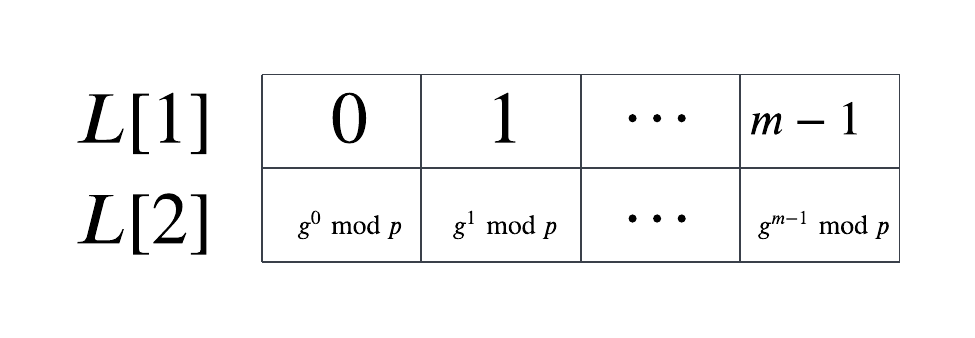
\includegraphics[width=\textwidth]{img/bsgs_L.png}
        \caption{The list $L$ that contains the pre-computed values of $g^{i}$.}
    \end{figure}
    \item The list is ordered by the values. Now, the ordered list will be referred as $L'$. This operation can be executed in $O(m \cdot \operatorname{log}(m) \cdot \operatorname{log}(p))$.
    \item The total cost of the "Baby Steps" part is then $O(m \cdot \operatorname{log}^{2}(p))$.
    \item[\textbf{Giant Steps}] This part consists in finding some $c_0, c_1$ such that $y = c_0 + m \cdot c_1$, given $m = \lceil \sqrt{p} \rceil$. This is done by iterating through the possible values of $c_1$ (\textbf{Giant Steps}), and trying at each iteration to find $c_0$ (\textbf{Baby Steps}).
    \item The first attempt is to find out if $x \in L'[2]$. This is accomplished by using the binary search algorithm, that terminates in $O(\operatorname{log}^{2}(p))$ (The number of iterations is $O(\operatorname{log}(m)) = O(\operatorname{log}(p))$, the comparisons cost $O(\operatorname{log}(p))$ each). If this is verified, then $y$ is the label of the element in $L'[2]$.
    \item The successive attempts try different values for $c_1$ such that:
    \[x \cdot g^{-c_1 \cdot m} \equiv_p g^{i}\]
    Therefore, if $x \cdot g^{-c_1 \cdot m} \in L'[2]$, there must be some $i$ such that $x \equiv_p g^{i + c_1 \cdot m}$. Needless to say, it turns out that $c_0 = i$, that is the label of the found element in $L'[2]$.
    \item The first values for $c_1$ is, trivially, $1$. This means that the first search will be conducted by using $x \cdot g^{-m}$. In order to optimize this, we can use the last value of $L$, that is $g^{m-1}$, and multiply it by $g$, obtaining then $g^m$. At this point, $g^{-m}$ can be found by applying the Extended Euclidean Algorithm.
    \item From this point on, the values of $c_1$ can be obtained by computing $g^{-i \cdot m} = g^{-m} \cdot g^{-(i - 1) \cdot m}$ at each step.
    \item The cost of this part, in the worst case, is $O(m \cdot \operatorname{log}^{2}(p))$, because for $m$ times the Binary search is executed. Fortunately, this formulation of the algorithm can terminate early.
\end{itemize}

\RestyleAlgo{ruled}
\begin{algorithm}
\KwData{$x \in \mathbb{Z}_{p}^{*}, g: <g> = \mathbb{Z}_{p}^{*}$}
\KwResult{$y: g^{y} \equiv_{p} x$}
\caption{Baby-steps/Giant-steps algorithm}\label{alg:baby_steps_giant_steps}
    \Comment{Baby steps part:}
    $c_{0}, c_{1} \gets 0, 0$\;
    $m \gets \lceil \sqrt{p} \rceil$\;
    $G \gets 1$\;
    $L \gets List(m - 1)$\;\Comment{List of $m - 1$ values}
    \For{$c_{i} \in \{0, \dots, m - 1\}$}{
        $G \gets g \cdot G \bmod p$\;
        $L[c_{i}] \gets (c_{i}, G)$\;
    }
    $L' \gets \operatorname{Sort}(L)$\;\Comment{Sorting by the values}
    \Comment{Giant steps part:}
    $G \gets g \cdot G \bmod p$\;\Comment{This is $g^{m} \bmod p$}
    $H \gets \operatorname{EEA}(G, p)$\;\Comment{This is $g^{-m} \bmod p$}
    \If{$x \in L'[2]$}{
        $c_{0} \gets \operatorname{Index}(L', x), 0$\;
        \Return{$c_{0} + c_{1} \cdot m$}\;
    }
    \Else{
        $h \gets x \cdot H$\;
        \For{$c_{1} = \{1, \dots, m - 1\}$}{
            \If{$h \in L'[2]$}{
                $c_{0} \gets \operatorname{Index}(L', x \cdot g^{-c_{1} \cdot m})$\;
                \Return{$c_{0} + c_{1} \cdot m$}\;
            }
            $h \gets h \cdot H \bmod p$\;
        }
    }
\end{algorithm}

\section{Index-Calculus Algorithm}
This algorithm tries to solve the discrete logarithm problem. In order to explain its inner workings, it's necessary to go through the concept of B-smoothness first.
\subsection{B-smoothness test}
The goal of this algorithm is to return $TRUE$ if and only if the input number $n$ is $B$-smooth, given $B$.

\RestyleAlgo{ruled}
\begin{algorithm}
\KwData{$n, B \in \mathbb{Z}$}
\caption{B-smoothness test}\label{alg:b_smoothness_test}
    $P \gets \{p_{i} : p_{i} \text{ is prime} \land p_{i} \leq B\}$\;
    $k \gets |P|$\;
    $N_{1} \gets n$\;
    $V = [0, \dots, 0]$\;
    $i \gets 1$\;
    \Do{$p_{i} \nmid N_{1}$}{\label{b_smt_2}
        \If{$p_{i} \mid N_{1}$}{
            $V[i] \gets V[i+1]$\;
            $N_{1} \gets \frac{N_{1}}{p_{i}}$\;
        }
    }
    \If{$N_{i} = 1$}{
        \Return{$TRUE$}\;
    }
    \If{$N_{1} > 1$}{
        $i \gets i + 1$\;
        \If{$i \leq k$}{
            \GoTo{\ref{b_smt_2}}\;
        }
        \Else{
            \Return{$FALSE$}\;
        }
    }
\end{algorithm}
Let's consider the cost of this algorithm in its worst case.\newline
The worst case is when $\forall i = 1, \dots, k: p_{i} \mid n$. Then
\begin{itemize}
    \item The cost of the division performed on \ref{b_smt_2} is $O(\operatorname{log}^{2}(n))$ b.o.
    \item The length of the loop at \ref{b_smt_2} is $O(\operatorname{log}(n))$, since:
    \[p_{i}^{\alpha_{i}} \leq n \land \alpha_{i} \leq \operatorname{log}(n) \implies \alpha_{i} \leq \frac{\operatorname{log}(n)}{\operatorname{log}(p_{i})}\]
    \item This process is repeated $k = \Pi(B)$ times, that is the number of prime numbers up to $B$.
    \item Therefore, the total cost of this algorithm is $O(\Pi(B) \operatorname{log}^{3}(n))$
\end{itemize}

\subsection{Index-Calculus algorithm}
Let $p$ be a prime number and $g: <g> = \mathbb{Z}_{p}^{*}$. The algorithm proceeds as follows:
\begin{itemize}
    \item[\textbf{Pre-computation}] This part of the algorithm prepares the values that will be used in the following steps of the algorithm.
    \item $B > 0 \in \mathbb{Z}$ is chosen, and the list of the prime numbers up to $B$ is computed. This can be achieved in $O()$ by using the Eratostene's sieve.
    \item $r > 0 \in \mathbb{N}$ is chosen, and $g^r \bmod p$ is computed. Then, if this result is B-smooth, is factorized in prime factors.
    \[g^{r} = p_{1}^{\alpha_{1, r}} \cdot p_{2}^{\alpha_{2, r}} \cdot \dots \cdot p_{k}^{\alpha_{k, r}}\]
    If $g^r \bmod p$ it's not B-smooth the process is repeated with a different $r$. Each attempt has a cost of $O(\operatorname{log}(r) \cdot \operatorname{log}^{2}(p))$. Remark that:
    \begin{align*}
        g^{\operatorname{log}_{g}(p_{i})} &\equiv_{p} p_{i}\\
        \implies r &\equiv_{p} \alpha_{1, r} \cdot \operatorname{log}_{g}(p_{1}) + \dots + \alpha_{k, r} \cdot \operatorname{log}_{g}(p_{k})\\
        \iff g^{r} &\equiv_{p} g^{\sum_{i=1}^{k} \alpha_{i, r} \cdot \operatorname{log}_{g}(p_{i})}
    \end{align*}
    \item This process is repeated $k$ times, in order to obtain the following system:
    \begin{align*}
        \begin{cases}
            r_{1} &\equiv_{p-1} \alpha_{1, r_{1}} \cdot \operatorname{log}_{g}(p_{1}) + \dots + \alpha_{k, r_{1}} \cdot \operatorname{log}_{g}(p_{k})\\
            r_{2} &\equiv_{p-1} \alpha_{1, r_{2}} \cdot \operatorname{log}_{g}(p_{1}) + \dots + \alpha_{k, r_{2}} \cdot \operatorname{log}_{g}(p_{k})\\
            \dots\\
            r_{k} &\equiv_{p-1} \alpha_{1, r_{k}} \cdot \operatorname{log}_{g}(p_{1}) + \dots + \alpha_{k, r_{k}} \cdot \operatorname{log}_{g}(p_{k})\\
        \end{cases}
    \end{align*}
    Consider now $M$, tha matrix of the coefficients $\{\alpha_{i, r_{j}}\}$, where $i,j = 1, \dots, k$. The Chinese Reminder Theorem states that there's a unique solution to this system in $\operatorname{log}_{g}(p_{i})$. This means that $\operatorname{det}(M) \neq 0$, and also $(\operatorname{det}(M), p-1) = 1$.
    \item At this point, we have $g, p, p_{i}, \operatorname{log}_{g}(p_{i})$ for $i = 1, \dots, k$.
    \item[\textbf{Computing DLOG(x)}] This part of the algorithm attemps to find the value of $y$ by using the values that were previously computed.
    \item This step consists in verifying if $x$ is $B$-smooth. That's because, if verified:
    \begin{align*}
        \exists \beta_{i}: x &\equiv_{p} \prod_{i=1}^{k} p_{i}^{\beta_{i}}\\
        \implies g^{y} &\equiv_{p} \prod_{i=1}^{k} g^{\operatorname{log}_{g}(p_{i}) \cdot \beta_{i}}\\
        \implies y &\equiv_{p - 1} \sum_{i=1}^{k} \operatorname{log}_{g}(p_{i}) \cdot \beta_{i}\\
    \end{align*}
    \item In case $x$ is not $B$-smooth, a number $s \in \{1, \dots, p-2\}$ can be generate. Let now be $x_{1} = x \cdot g^{s} \bmod p$. If $x_{1}$ is not $B$-smooth, pick another $s$. If it is, we have that:
    \begin{align*}
        \exists \beta_{i}: x_{1} &\equiv_{p} \prod_{i=1}^{k} p_{i}^{\beta_{i}}\\
        \implies g^{y + s} &\equiv_{p} \prod_{i=1}^{k} g^{\operatorname{log}_{g}(p_{i}) \cdot \beta_{i}}\\
        \implies y + s &\equiv_{p - 1} \sum_{i=1}^{k} \operatorname{log}_{g}(p_{i}) \cdot \beta_{i}\\
    \end{align*}
    Since we generated $s$, we can now easily determine $y$.
\end{itemize}

\section{Pollard's Rho-method for the Discrete Logarithm Problem}
\subsection{General idea}
This algorithm provides a probabilistic solution to the Discrete Logarithm problem, by applying the same idea that is applied to the Factoring Problem.\newline
Consider what follows:
\begin{itemize}
    \item Let $G = <g> = \mathbb{Z}_{p}^{*}$ and $|G| = m \in \mathbb{N}$.
    \item Let also be $x \equiv_{G} g^{y}$, with $y$ unknown.
    \item $G$ is partitioned in 3 subsets, as follows:
    \begin{itemize}
        \item $G_1 = \{a \in \mathbb{Z}_{p}^{*}: 0 < a < \frac{p}{3}\}$
        \item $G_2 = \{a \in \mathbb{Z}_{p}^{*}: \frac{p}{3} \leq a < \frac{2p}{3}\}$
        \item $G_3 = \{a \in \mathbb{Z}_{p}^{*}: \frac{2p}{3} \leq a\}$
    \end{itemize}
    \item Let $f: G \rightarrow G$, such that:
    \begin{align*}
        f(a) &=
        \begin{cases}
            g \cdot a \text{ if } a \in G_1 \\
            a^2 \text{ if } a \in G_2 \\
            x \cdot a \text{ if } a \in G_3 \\
        \end{cases}
    \end{align*}
    \item Consider that $f^{(k)}(a_0) = f \circ f \circ \dots \circ f$, $k$ times. Remark that $a_0 \in G$ is chosen randomly.
    \item The algorithm tries to find some $h, k$ such that $f^{(k)}(a_0) =_{G} f^{(h)}(a_0)$. This is achieved in the same way as the one for the Factoring Problem, by iterating $f(f^{(k - 1)}(a_0))$ and $f(f(f^{(k - 1)}(a_0)))$.
    \item Remark that $\forall k \geq 0, \exists i_{k}, j_{k} \in \mathbb{N}: f^{(k)}(a_0) = x^{i_k} \cdot g^{j_k}$. This is because $a_0 \in G \iff a_0 = g^{j_0}$. Then, we have that:
    \begin{align*}
        (i_{k+1}, j_{k+1}) &=
        \begin{cases}
            (i_{k}, (j_{k} + 1) \bmod m) \cdot a \text{ if } f^{(k)}(a_0) \in G_1 \\
            (2i_{k} \bmod m, 2j_{k} \bmod m) \text{ if } f^{(k)}(a_0) \in G_2 \\
            ((i_{k} + 1) \bmod m, j_{k}) \cdot a \text{ if } f^{(k)}(a_0) \in G_3 \\
        \end{cases}
    \end{align*}
    \item When we find some $f^{(k)}(a_0) = f^{(h)}(a_0)$, we can use this relationship as follows:
    \begin{align*}
        f^{(k)}(a_0) &= f^{(h)}(a_0)\\
        x^{i_k} \cdot g^{j_k} &=_G x^{i_h} \cdot g^{j_h}\\
        g^{j_k - j_h} &=_G x^{i_k - j_h} =_G g^{y \cdot (i_k - i_h)}\\
        j_k - j_h &\equiv_{m} y \cdot (i_k - i_h)\\
        \text{If } (i_k - i_h, m) = 1 \text{ then, } y \equiv_{m} (j_k - j_h) \cdot (i_k - i_h)^{-1}\\
        \text{If } (i_k - i_h, m) = d > 1 \text{ then, } y \cdot (i_k - i_h) \equiv_{m} (j_k - j_h)\\
        \text{Reduced congruence:}\\
        y \cdot (\frac{i_k - i_h}{d}) &= (\frac{j_k - j_h}{d}) \bmod \frac{m}{d}\\
        \implies (\frac{i_k - i_h}{d}, \frac{m}{d}) &= 1\\
        \text{Therefore, } y &= (\frac{j_k - j_h}{d}) \cdot (\frac{i_k - i_h}{d}) \bmod \frac{m}{d}
    \end{align*}
    At this point, verify that $g^y \equiv_m x$. If it doesn't work, try:
    \[g^{y + \mathcal{l} \cdot (\frac{m}{d}), \text{ where } \mathcal{l} \in \{0, 1, \dots, d - 1\}}\]
\end{itemize}

\subsection{Floyd's iteration}
This method, as its correspondant for the Factoring Problem, aims to optimize the research for the collisions.
\begin{itemize}
    \item Assume that you have found some $m_0 < l_0$ such that $f^{(m_0)}(a_0) = f^{(l_0)}(a_0)$. Then, let $\mu = l_0 - m_0$.
    \item Then, you'll have that $f^{(m)}(a_0) = f^{(l)}(a_0) \implies l \equiv_{\mu} m$.
    \item Let now $z = \mu \cdot \lceil \frac{m_0}{\mu} \rceil$ and let $2z = z + \mu \cdot \lceil \frac{m_0}{\mu} \rceil$. Then $f^{(z)}(a_0) = f^{(2z)}(a_0)$.
    \item Let now $H_{1}(s) = f^{(s)}(a_0)$, $H_{2}(s) = f^{(2s)}(a_0)$ and
    $H_{1}(s + 1) = f(H_{1}(s))$, $H_{2}(s + 1) = f(f(H_{2}(s)))$
    \item This allows to spare some computation steps, since we're only looking for meaningful collisions after we've found the first one. This means that we must perform only $O(\sqrt{m})$ steps in order to have a probability of $\frac{1}{2}$ to find $y$.
\end{itemize}

\section{Chaum-van Heijst-Pfitzmann compression function}
Consider the following:
\begin{itemize}
    \item Let $p, q$ be two prime numbers such that $p \equiv 3 \bmod 4$ and $q = \frac{p-1}{2}$.
    \item Let $<g> = \mathbb{Z}_{p}^{*}$, and $t \in \mathbb{Z}_{p}^{*}$.
\end{itemize}
The hash function $h$ is defined as
\begin{align*}
    h: \mathbb{Z}_{q} \times \mathbb{Z}_{q} &\rightarrow \mathbb{Z}_{p}^{*}\\
    h(a, b) &= g^{a} \cdot t^{b} \bmod p
\end{align*}
The signature of the cleary states that the input's size is reduced of a factor 2. Let's see why:
\begin{align*}
    \operatorname{Size}((a,b)) &= 2 \cdot \operatorname{log}(q)\\
    = 2 \cdot \operatorname{log}(\frac{p-1}{2}) &= 2 \cdot (\operatorname{log}(p-1) - \operatorname{log}(2))\\
    &= 2 \cdot \operatorname{log}(p \cdot (1 - \frac{1}{p})) - 2 \cdot \operatorname{log}(2)\\
    &= 2 \cdot \operatorname{log}(p) + 2 \cdot \operatorname{log}(1 - \frac{1}{p})) - 2 \cdot \operatorname{log}(2)\\
    &= 2 \cdot \operatorname{log}(p) - 2 \cdot \operatorname{log}(2) + O(\frac{1}{p}) \text{, Since } \operatorname{log}(1 - \frac{1}{p}) = O(\frac{1}{p})
\end{align*}
Therefore, $\operatorname{Size}((a,b))$ is approximately twice the size of the output, that is $O(\operatorname{log}(p))$.\newline
What follows is the proof that the security of this hash function stands on the hardness of the Discrete Logarithm Problem.
\begin{itemize}
    \item
\end{itemize}
